\documentclass[hidelinks,12pt]{article}
\usepackage[utf8]{inputenc}
\usepackage{mathtools}
\usepackage{amsthm}
\usepackage{amsmath}
\usepackage{amsfonts}
\usepackage{amssymb}
\usepackage{centernot}
\usepackage{marvosym}
\usepackage{enumitem}
\usepackage{hyperref}
\usepackage{graphicx}
\graphicspath{{/home/theo/Documents/GitHub/Math-Homeworks/Images/}}
\setcounter{tocdepth}{1}
\let\marvosymLightning\Lightning
\renewcommand{\geq}{\geqslant}
\renewcommand{\leq}{\leqslant}
\newtheorem{theorem}{Theorem}
\newtheorem{corollary}{Corollary}[theorem]
\newtheorem*{remark}{Remark}
\newcommand{\R}{\mathbb{R}}
\newcommand{\N}{\mathbb{N}}
\newcommand{\Z}{\mathbb{Z}}
\newcommand{\Q}{\mathbb{Q}}
\newcommand{\F}{\mathbb{F}}
\newcommand{\divby}{%
  \mathrel{\text{\vbox{\baselineskip.65ex\lineskiplimit0pt\hbox{.}\hbox{.}\hbox{.}}}}%
  }
\newcommand{\notdivby}{\centernot\divby}
\title{\scalebox{2}{Math 835 Homework 1}}
\author{\scalebox{1.5}{Theo Koss}}
\date{September 2024}

\begin{document}

\maketitle
\section{Chapter 13}
\subsection{Chapter 1}
\begin{enumerate}
	\item[1.] Show that $p(x)=x^3+9x+6$ is irreducible in $\Q[x]$. Let $\theta$ be a root of $p(x)$, find the inverse of $1+\theta$ in $\Q(\theta)$.
		\begin{proof}
			By the Eisenstein criterion, let $p=3$, $p\mid 9$ and $p\mid 6$ but $p^2=9\centernot\mid 6$ and $p\centernot\mid 1$.
		\end{proof}
		Following example 4 in 13.1, (pp. 515), apply Euclidean Algorithm in $\Q[x]$ to get $a(x)$ and $b(x)$ such that \[a(x)(1+x)+b(x)(x^3+9x+6)=1\]
		\begin{centering}{\scalebox{.75}{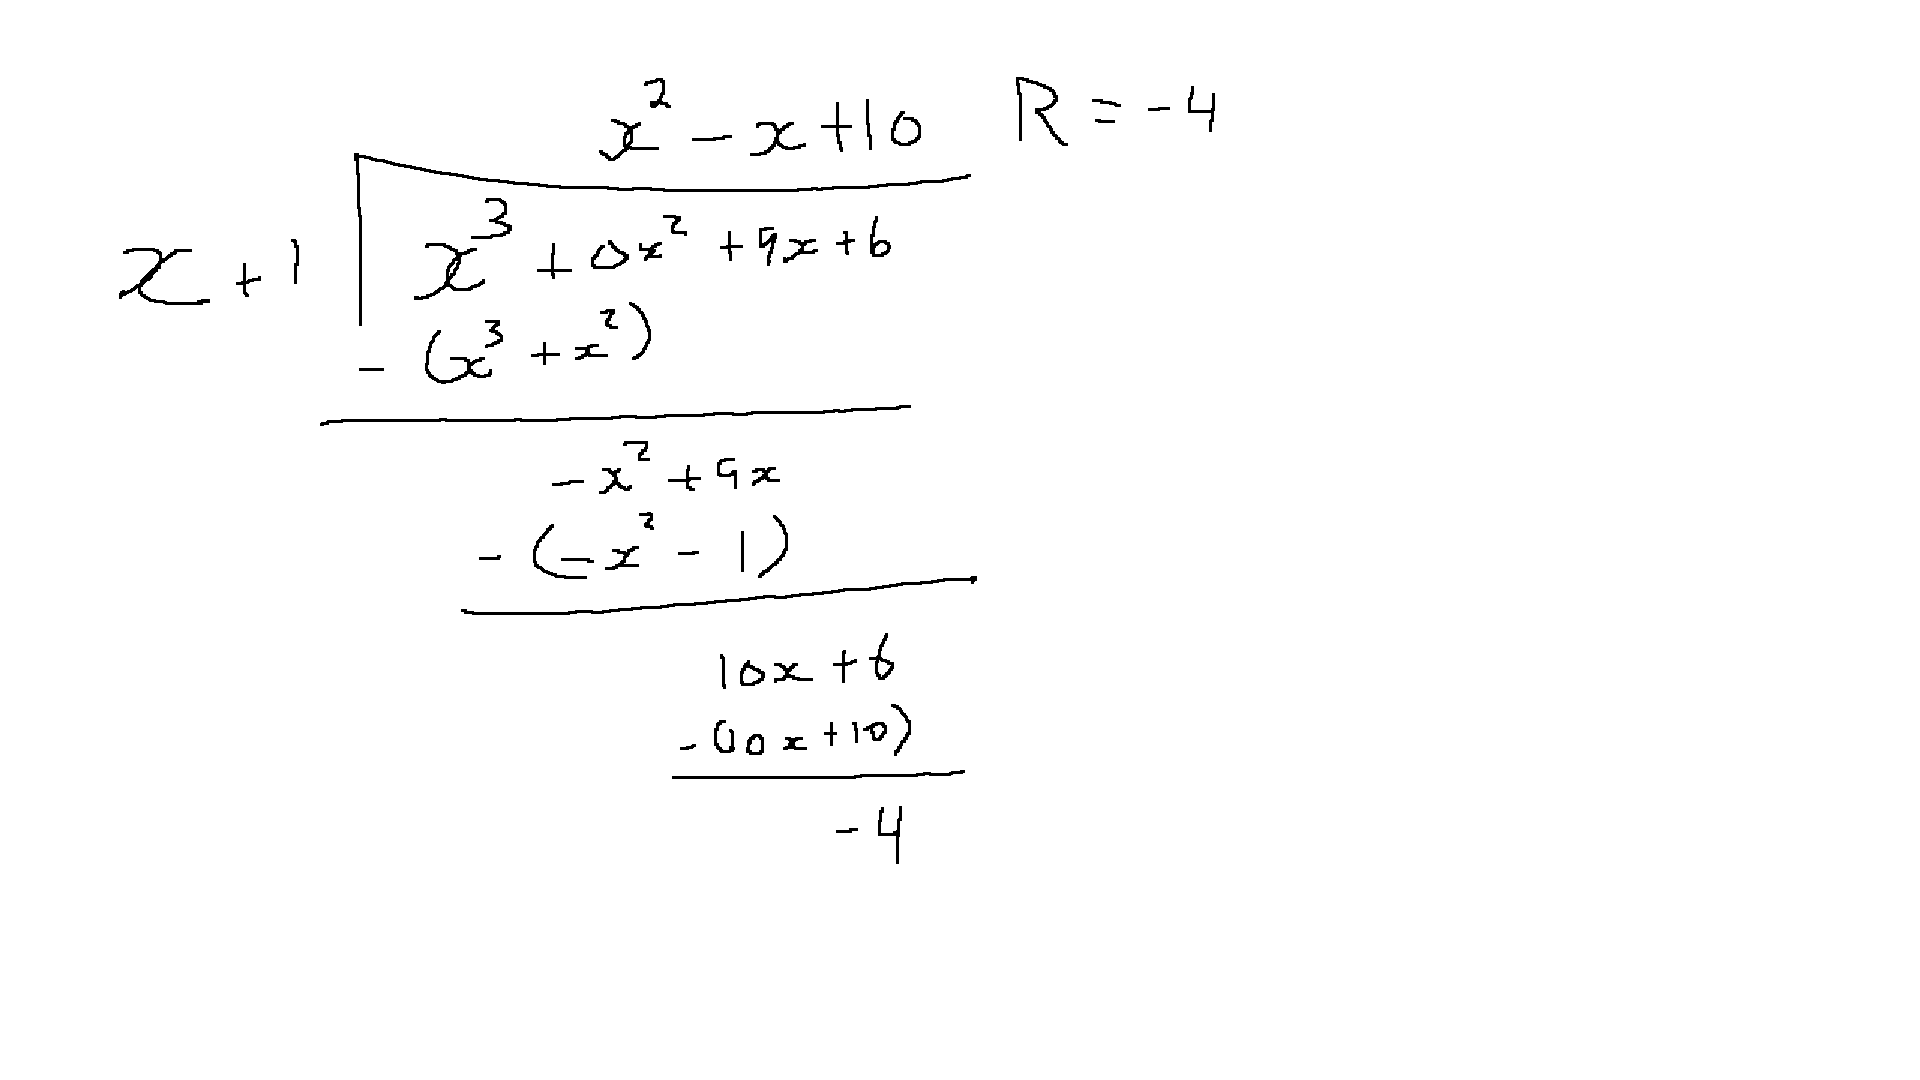
\includegraphics{LongDiv.png}}}\\\end{centering}
		\begin{align*}
			a(x)=\frac{(x^2-x+10)}{4},\ b(x)         & =-\frac{1}{4}\tag{Div. both sides by 4} \\
			\frac{(1+x)(x^2-x+10)-(x^3+9x+6)}{4}     & =1                                      \\
			\frac{(1+\theta)(\theta^2-\theta+10)}{4} & =1\tag{Since $p(\theta)=0$}             \\
			\implies (1+\theta)^{-1}                 & =\frac{\theta^2-\theta+10}{4}
		\end{align*}
	\item[3.] Show that $x^3+x+1$ is irreducible over $\F_2$ and let $\theta$ be a root. Compute the powers of $\theta$ in $\F_2$.
		\begin{proof}
			$p(x)=x^3+x+1$ is irreducible by the rational root theorem, and checking $p(0)=0^3+0+1\neq0$ and $p(1)=1^3+1+1\neq0$.
		\end{proof}
		Powers of $\theta$:
		\begin{align*}
			\theta^1 & =\theta                              \\
			\theta^2 & =\theta^2                            \\
			\theta^3 & =\theta+1                            \\
			\theta^4 & =\theta^2+\theta                     \\
			\theta^5 & =\theta^3+\theta^2=\theta^2+\theta+1 \\
			\theta^6 & =\theta^2+1                          \\
			\theta^7 & =1=\theta^0                          \\
			         & \vdots                               \\
		\end{align*}
\end{enumerate}
\end{document}
